%*****************************************
\chapter{Functional testing for the mean}\label{ch:functional-testing}
%*****************************************

\begin{flushannotation}
  {This chapter is partially based on the preprint
  ``A Bayesian one-sample test for the mean of functional data''
  \citep{berrendero2026bayesian}.}
\end{flushannotation}

\note{Revisar todos los productos escalares L2 que sean con el subíndice 2}

\noindent A core problem in statistics involves hypothesis testing for quantities of interest. As such, considerable efforts have been devoted to generalizing frequentist two-sample tests \citep{fan1998test,hall2007two,zhang2010two}, analysis of variance methods \citep{cuevas2004anova, cuesta2010simple, zhang2013analysis}, change point detection procedures \citep{berkes2009detecting,hormann2010weakly}, repeated measures analysis \citep{martinez2011repeated,smaga2020note} or dependence tests in linear regression \citep{cardot2003testing,kokoszka2008testing} to functional data, providing \(p\)-values and decision rules based on asymptotic approximations or bootstrap resampling. However, the conceptually simpler one-sample tests, often used to detect the presence or absence of a certain effect within a given population, have received less attention in the FDA literature. Notable exceptions include proposals by \citet{mas2007testing}, \citet{munk2008one} and \citet{zhang2013analysis}, where the authors explore different tests for the mean of a functional sample.

On the other hand, Bayesian methods for hypothesis testing---introduced in modern form by \citet{jeffreys1961theory}---are extensively studied and applied in multivariate settings, offering a principled alternative to the often criticized \(p\)-value approach \citep[see][and references therein for a general overview]{robert2007bayesian, robert202250}. However, despite their broad adoption, they remain comparatively underdeveloped within the FDA framework. We aim to bridge this gap by proposing a Bayesian test for the mean function \(\mu\) of a Gaussian process observed through i.i.d.\ samples, which serves as a building block for more complex statistical analyses and machine learning applications. In particular, we provide a method for testing the point-null hypothesis \(H_0: \mu \equiv \mu_0\) versus the composite alternative \(H_1: \mu \not\equiv \mu_0\), where \(\mu_0(\cdot)\) is a predetermined function. We focus on the simple hypothesis of exact equality, in contrast to \textit{precise} or \textit{relevant} hypotheses such as \(H_0^\epsilon: \|\mu-\mu_0\| < \epsilon\) for a given \(\epsilon>0\). Although these precise hypothesis may be useful when an exact zero is not meaningful or reasonable, in a Bayesian framework they can be conceptually encoded in the corresponding point-null hypothesis via prior beliefs, as argued by \citet{berger1987testing}. The proposed test is based on the Bayes factor
\[
\bff_{10} = \frac{\pp(\text{data}|H_1)}{\pp(\text{data}|H_0)},
\]
which measures the evidence for \(H_1\) over \(H_0\) and is linked to the prior and posterior odds through the formula
\[
\frac{\pp(H_1|\text{data})}{\pp(H_0|\text{data})} = \bff_{10} \, \times\, \frac{\pp(H_1)}{\pp(H_0)}.
\]
Using Bayes factors to quantify the evidence against the null hypothesis in a continuous manner is the standard approach in Bayesian testing, popularized since the seminal work by \citet{kass1995bayes}. Because they are intimately related to the posterior probability of the null, Bayes factors provide a direct probabilistic way of interpreting the test decision, while also allowing the incorporation of prior information. Moreover, despite being a loose analog of a likelihood ratio test, the Bayes factor \(\bff_{10}\) can be inverted to provide evidence in favor of \(H_0\), which is not possible in frequentist tests due to the built-in asymmetry. 

Most functional tests in the literature employ some form of dimension reduction via projections or basis expansions as a first step. However, we take a slightly different approach and follow earlier work by \citet{berrendero2018use,berrendero2025bayesian}. In particular, we directly assume that the mean function is a member of the reproducing kernel Hilbert space (RKHS) associated with the covariance function of the underlying Gaussian process, so that it can be approximated via a finite linear combination of kernel sections. We will see that this assumption is reasonable and allows us to completely specify a Bayesian test, circumventing the difficulty of placing a prior distribution on an infinite-dimensional space, and providing a closed-form likelihood expression via Radon--Nikodym derivatives. Since we do not restrict ourselves to conjugate models, we use the reversible jump variant of Markov chain Monte Carlo methods (RJMCMC), proposed by \citet{green1995reversible}, to approximate the posterior distribution. From this approximation we obtain estimators of the posterior probability of the null hypothesis and the Bayes factor, which can be used to guide decision-making while explicitly accounting for uncertainty.

To validate the methodology from a theoretical point of view, we study the large-sample consistency of our test and measure the speed of posterior concentration. This technique has become a standard tool in the frequentist assessment of Bayesian procedures, as exemplified by the highly relevant work of \citet{ghosal2017fundamentals}. Posterior consistency of the Bayes factor in a point-null testing situation was established by \citet{dass2004note}, but their abstract approach cannot provide posterior contraction rates. As a novel contribution, we show that under \(H_0\) the posterior probability of the alternative goes to zero at a polynomial rate, while under \(H_1\) the posterior probability of the null decays exponentially fast. On the other hand, finite-sample performance is evaluated by numerical simulations in terms of frequentist metrics, such as type I error (false positive rate), type II error (false negative rate) or power (true positive rate).

%%%%%%%%%%%%%%%%%
%break

Let \(X_{1:n}=(X_1,\dots, X_n)\) be an i.i.d.\ sample of a Gaussian process \(X\sim \gp(\mu, K)\) with mean \(\mu\) and strictly positive definite covariance function \(K\), which is assumed to be known for the time being. Without loss of generality we set \(\mu_0\equiv 0\) and \(T=1\), which leads us to consider the hypotheses
\[
H_0: \mu(t)=0 \text{ for all } t \in [0,1] \quad \text{against} \quad H_1: \mu(t)\neq 0 \text{ for some } t \in [0,1].
\]

Our key modeling assumption is that \(\mu\in\Hcal(K)\). Not only is this space naturally linked to the process \(X\), but in general it contains smoother functions than, say, \(L^2[0,1]\). More importantly, it provides a direct finite-dimensional representation of the mean function if we further suppose that \(\mu\in\Hcal_0(K)\), which is dense in \(\Hcal(K)\) by construction. Indeed, we propose a parametric model (with a functional interpretation) based on the approximation
\begin{equation}\label{eq:mu-h0}
\mu_\theta(\cdot) = \sum_{j=1}^p \beta_j K(t_j, \cdot),
\end{equation}
where \(\theta=(p, \tau_p, b_p)\) is a generic parameter, with \(\tau_p=(t_1,\dots, t_p)\in [0,1]^p\) the time instants, \(b_p=(\beta_1,\dots,\beta_p)\in \R^p\) the coefficients and \(p\in\N\) the dimensionality (which is not fixed). We will omit the subscript \(p\) when it is understood from context, and assume that the grid of observation \(\mathcal S\) is fine enough to contain all the relevant time instants.

Note that when \(K\) is strictly positive definite, the null hypothesis \(\mu_\theta\equiv 0\) corresponds to \(b=0\) as long as the time instants are distinct. Thus, the parameter spaces for the null and alternative hypotheses in our Bayesian test are
\[
\Theta_0=\bigcup_{p\in\N}\{b \in \R^p: b=0\}\quad \text{and}\quad \Theta_1=\bigcup_{p\in\N}\{(p, \tau, b): \tau \in \mathcal T_p,\, b \in \R^p\setminus \{0\}\},
\]
respectively, where \(\mathcal T_p = \{(t_1,\dots,t_p)\in [0,1]^p: t_1 < \cdots < t_p\}\) is the ordered unit simplex. Although not strictly needed, we impose an ordering constraint to avoid identifiability issues and reduce the parameter space by a factor of \(p!\) on each dimension.

\subsection{Likelihood and Prior Distributions} 

Let \(\pp_\mu\) be the distribution of \(\gp(\mu, K)\) on the sample space \(\mathcal C[0,1]\) (continuous functions on \([0,1]\)), and similarly let \(\pp_0\) be the distribution of \(\gp(0, K)\). Since both distributions are Gaussian with common covariance, the Feldman--Hájek dichotomy \citep{feldman1958equivalence} implies that \(\pp_\mu\) is absolutely continuous with respect to \(\pp_0\) whenever \(\mu\in\Hcal(K)\), which is precisely our assumption on the mean function. In this situation, the density of \(\pp_{\mu_\theta}\) with respect to \(\pp_0\) is given by \citep[Theorem 1]{berrendero2018use}
\begin{equation}\label{eq:rn-derivative}
  \frac{d\pp_{\mu_\theta}}{d\pp_0}(X) = \exp\left\{\langle X, \mu_\theta\rangle_K - \frac{1}{2}\|\mu_\theta\|^2_K\right\}.
\end{equation}
In a Bayesian setting, this Radon--Nikodym derivative can be interpreted as the likelihood \(L(X|\theta)\) of observing a path \(X\) under the parameter \(\mu_{\theta}\), with respect to the common reference measure \(\pp_0\). Now, since \(\mu_{\theta}\) has the finite-dimensional representation~\eqref{eq:mu-h0}, we can evaluate the scalar product (via Loève's isometry) and the RKHS norm, obtaining closed-form expressions \(\langle X, \mu_\theta\rangle_K = \sum_{j=1}^p \beta_j X(t_j)\) and \(\|\mu_\theta\|^2_K = \sum_{j=1}^p \sum_{k=1}^p \beta_j\beta_k K(t_j, t_k)\). In particular, for our i.i.d.\ sample the joint likelihood becomes
\begin{equation}\label{eq:likelihood}
  L(X_{1:n}| p, \tau, b) = \exp\left\{S_n(\tau)'b - \frac{n}{2}b' K_{\tau} b\right\},
\end{equation}
where \(S_n(\tau)=\sum_{i=1}^n (X_i(t_1), \dots, X_i(t_p))'\) and \(K_{\tau}=[K(t_j, t_k)]_{j,k=1}^p\). Then, for \(\theta=(p,\tau,b)\) we consider the parametric hierarchical model
\[
  X_1,\dots, X_n | \theta \stackrel{\text{i.i.d.}}{\sim} \gp(\mu_\theta, K),\quad
  p \sim \Pi(p),\quad \tau|p \sim \Pi(\tau|p),\quad b|p \sim \Pi(b|p),
\]
where the implied independence between \(\tau\) and \(b\) (given \(p\)) is just a convenience. We impose a discrete prior distribution \(\Pi(p)\) on the number of components, and a continuous distribution \(\Pi(\tau|p)\) for the time instants (e.g.\ uniform on \(\mathcal T_p\)). The prior on the coefficient vector \(b\) has to be chosen carefully, since any continuous distribution will give zero mass to the null event \(\{b=0\}\). To remedy this, we follow a \textit{spike-and-slab} approach reminiscent of Bayesian variable selection in linear regression \citep[e.g.][]{mitchell1988bayesian,ishwaran2005spike}, whereby a fixed mass is assigned to the null hypothesis and the remaining mass is distributed continuously on the alternative. Let \(0<\pi_0<1\) be the prior belief that the null hypothesis is true, and consider
\begin{equation}\label{eq:prior-b}
\Pi(b|p) = \pi_0\Pi_{\text{spike}}(b) + (1-\pi_0)\Pi_{\text{slab}}(b) = \pi_0 \delta_0(b) + (1-\pi_0)\mathcal N_p(b|0, \eta^2 I_p),
\end{equation}
where \(\delta_0\) is a Dirac measure at \(0\) (the ``spike''), \(I_p\) is the identity matrix of order \(p\), and \(\eta^2>0\) is a scalar hyperparameter. Unlike the priors for \(p\) and \(\tau\), the choice of a normal distribution for the ``slab'' prior of \(b\) is not arbitrary; it will be used as a conjugacy device to simplify the posterior distribution later on. Note that this construction induces the priors \(\Pi(H_0)=\pi_0\) and \(\Pi(H_1)=1-\pi_0\), since the null hypothesis is reinterpreted as \(H_0: b=0\).

\subsection{Posterior Approximation} 

Bayes' formula gives a posterior distribution \(\Pi_n(p, \tau, b | X_{1:n}) \propto \Pi(p, \tau, b)L(X_{1:n}|p, \tau, b)\) up to a multiplicative constant, which can be approximated through computational methods. However, sampling the high-dimensional parameter \(b\in \R^p\) is notoriously challenging, so we marginalize it analytically thanks to the prior structure in~\eqref{eq:prior-b}. The marginal likelihood has the form
\begin{align*}
  m(X_{1:n}|p, \tau) &= \pi_0\int \Pi_{\text{spike}}(b)L(X_{1:n}|p, \tau, b)\, db + (1-\pi_0)\int \Pi_{\text{slab}}(b)L(X_{1:n}|p, \tau, b)\, db\\
  &= \pi_0m_{\text{spike}}(X_{1:n}|p, \tau) + (1-\pi_0)m_{\text{slab}}(X_{1:n}|p, \tau).
\end{align*}
Since \(\Pi_{\text{spike}}\) is a point mass at \(b=0\), we have \(m_{\text{spike}}(X_{1:n}|p,\tau)=e^0=1\), according to~\eqref{eq:likelihood}. In the slab part we get an exact integral, applying the formula for the moment generating function (at \(t=1\)) of a quadratic form in Gaussian variables \citep[Corollary 3.2a.1]{mathai1992quadratic}:
\begin{equation}\label{eq:m-slab}
  \begin{split}
  m_{\text{slab}}(X_{1:n}|p, \tau) &= \int \mathcal N_p(b|0, \eta^2 I_p)\exp\left\{S_n(\tau)'b - \frac{n}{2}b' K_{\tau} b\right\}\, db \\
  &= \eta^{-p} |\Lambda_\tau|^{-1/2}\exp\left\{\frac{1}{2}S_n(\tau)' \Lambda_\tau^{-1}S_n(\tau)\right\},
  \end{split}
\end{equation}
where \(\Lambda_\tau = nK_\tau + \eta^{-2}I_p\). All in all, the marginal posterior expression becomes
\begin{equation}\label{eq:posterior-p-tau}
\Pi_n(p, \tau|X_{1:n}) \propto \Pi(p)\Pi(\tau|p)[\pi_0 + (1-\pi_0)m_{\text{slab}}(X_{1:n}|p, \tau)].
\end{equation}

At this point we choose to use the RJMCMC algorithm to approximate the marginal posterior \(\Pi_n(p, \tau|X_{1:n})\). Unlike standard MCMC approaches, this method can traverse a variable-dimension parameter space by proposing the birth of a new component or the death of an existing one at each iteration. This yields a sequence of approximate posterior draws \(\{(p^{(r)}, \tau^{(r)}): r=1,\dots,R\}\), possibly of different dimensions. We can subsequently reapply Bayes' formula conditional on \((p^{(r)},\tau^{(r)})\) to recover the posterior samples \(b^{(r)}\), which in turn can be used to construct posterior samples \(\mu^{(r)}\) of the mean function via~\eqref{eq:mu-h0}. Details on these calculations and the specific implementation of RJMCMC are given in Appendix~\ref{app:rjmcmc}.

\subsection{Decision Criteria} One of the main advantages of our Bayesian framework is that it naturally provides several posterior metrics to evaluate the evidence against the null hypothesis given the data. As we said before, the posterior probability of the null, \(\Pi_n(b=0|X_{1:n})\), corresponds to \(\E[\mathds{1}\{b=0\}|X_{1:n}]\), where \(\mathds{1}\{\cdot\}\) is the indicator function. We could naively compute the estimator \(R^{-1}\sum_{r} \mathds{1}\{b^{(r)}=0\}\) with our posterior samples, which by the ergodic properties of the RJMCMC sampler would indeed converge almost surely to the target probability (under standard assumptions). However, this estimator introduces the Monte Carlo noise of actually sampling \(b^{(r)}\), which is not desirable. Instead, we can consider the conditional posterior probability of the spike (computed through Bayes' formula)
\begin{equation}\label{eq:psi-posterior-spike}
\psi_n(p,\tau) = \Pi_n(b=0|p,\tau, X_{1:n}) = \frac{\pi_0}{m(X_{1:n}|p,\tau)},
\end{equation}
and use the equivalence
\[
 \E[\psi_n(p,\tau)|X_{1:n}] = \sum_p \int_{\mathcal T_p} \psi_n(p,\tau) \Pi_n(p,\tau|X_{1:n})\, d\tau = \Pi_n(b=0|X_{1:n})
\]
to obtain a more efficient estimator of the posterior probability of \(H_0\). Indeed, by the law of total variance we have:
\[
\var(\psi_n(p,\tau)|X_{1:n}) = \var(\E[\mathds{1}\{b=0\}|p, \tau, X_{1:n}]|X_{1:n}) \leq \var(\mathds{1}\{b=0\}|X_{1:n}).
\]
Hence, conditioning on \((p,\tau)\) and averaging the posterior spike probabilities \(\psi_n(p^{(r)}, \tau^{(r)})\) instead of the raw indicators \(\mathds{1}\{b^{(r)}=0\}\) yields the improved estimator\footnote{This strategy is similar to the Rao-Blackwellization process to reduce the variance of an estimator \citep[Theorem 7.9]{ghosh2006introduction}.}
\[
\hat \pi_{\text{null}} = \frac{1}{R}\sum_{r=1}^R \psi_n(p^{(r)}, \tau^{(r)}).
\]
Under the 0--1 loss function, we would reject the null hypothesis if \(\hat \pi_{\text{null}} \leq 1/2\) and accept it otherwise, but practitioners can fix any arbitrary threshold on a case-by-case basis.

Another quantity of interest to assess the evidence against the null hypothesis is the Bayes factor, which is defined as
\[
\bff_{10}(X_{1:n}) = \frac{L(X_{1:n}|H_1)}{L(X_{1:n}|H_0)} = \frac{1 - \Pi_n(H_0|X_{1:n})}{\Pi_n(H_0|X_{1:n})} \cdot \frac{\pi_0}{1-\pi_0}
\]
and represents the evidence in favor of \(H_1\) over \(H_0\) as supported by the data. For example, if \(\pi_0=1-\pi_0=1/2\), then \(\Pi_n(H_0|X_{1:n})=1/2\) corresponds to \(\bff_{10}(X_{1:n}) = 1\). Note that in our model \(L(X_{1:n}|H_0)\) is actually equal to 1 by construction, since we take \(\pp_0\) as the reference measure. In practice, we report an estimated Bayes factor 
\[
\hat{\bff}_{10} = \frac{1 - \hat \pi_{\text{null}}}{\hat \pi_{\text{null}}}\cdot \frac{\pi_0}{1-\pi_0}
\]
and use Jeffreys' scale (see Table~\ref{tab:jeffreys-scale}) to weigh the evidence against \(H_0\). Observe that the Bayes factor (a likelihood ratio) is actually independent of the prior belief \(\pi_0\), so it acts as a somewhat more objective measure to compare evidence against \(H_0\) across different models.

\begin{table}[t]
  \centering
  %\small
  \setlength{\tabcolsep}{7pt}
  \renewcommand{\arraystretch}{1.05}
  \begin{tabular}{@{}rrl@{}}
  \midrule
   \multicolumn{1}{c}{\(\bff_{10}\)} & \multicolumn{1}{c}{\(\log \bff_{10}\)} & \multicolumn{1}{c@{}}{Strength of evidence against \(H_0\)} \\
  \midrule
  \(<1\) & \(<0\) & Negative\\
  1 to 3 & 0 to 1.1 &  Barely worth mentioning \\
  3 to 20 & 1.1 to 3 & Positive \\
  20 to 150 & 3 to 5 & Strong \\
  \(> 150\) &  \(>5\) & Very strong \\[.5ex]
  \midrule
  \end{tabular}
  \caption{Jeffreys' scale for the Bayes factor, adapted by \citet{kass1995bayes}.}\label{tab:jeffreys-scale}
\end{table}

Lastly, we can report the posterior probability of the so-called region of practical equivalence (ROPE), defined for a small \(\epsilon > 0\) as 
\[
\Pi_n\left(\sup_s |\mu(s)| < \epsilon \mid X_{1:n}\right).
\]
This ``practical null'' probability is sometimes used to evaluate \(H_0\) when an exact zero is not meaningful, and is readily available in our Bayesian setting without changing the overall approach (i.e.\ without considering a precise hypothesis \(H_0^\epsilon:\sup_s|\mu(s)| < \epsilon\) from the start). The easiest way to approximate the ROPE probability on the observation grid \(\mathcal S\) is through the Monte Carlo estimator
\[
\hat\pi_{\text{ROPE}}(\epsilon) = \frac{1}{R}\sum_{r=1}^R \mathds{1}\left\{\max_{s\in\mathcal S} |\mu^{(r)}(s)| < \epsilon\right\}.
\]

\subsection{Posterior Summaries and Uncertainty Quantification}\label{sec:posterior-summaries}

An additional benefit of the Bayesian framework is that it facilitates posterior inference on the mean function as a by-product of the testing procedure. For example, we can estimate the posterior mean function \(\mu^{\text{PM}}(\cdot)=\E[\mu(\cdot)|X]\) using the conditional expectation strategy again, which is typically much less noisy than averaging posterior draws \(\mu^{(r)}\) directly. Indeed, for a fixed \(s\in[0,1]\) the law of total expectation gives \(\E[\mu(s)|X] = \E[\E[\mu(s)|p, \tau, X]|X]\), and the same variance reduction argument as before applies. In the i.i.d.\ case, the inner posterior expectation admits the closed-form expression 
\[
\E[\mu(s)|p, \tau, X_{1:n}] = (1-\psi_n(p, \tau))K(\tau, s)'m_b(\tau),
\]
where \(K(\tau, s)\) denotes the \(p\times 1\) vector with entries \(K(t_j, s)\), and \(m_b(\tau) = \Lambda_\tau^{-1}S_n(\tau)\) is the posterior expectation of the coefficients under the slab (see Appendix~\ref{app:rjmcmc}). Consequently, a Monte Carlo estimator of the posterior mean function is given by
\[
\hat\mu_n^{\text{PM}}(\cdot) = \hat{\E}[\mu(\cdot)|X_{1:n}]=\frac{1}{R} \sum_{r=1}^R (1-\psi_n(p^{(r)}, \tau^{(r)}))K(\tau^{(r)}, \cdot)'m_b(\tau^{(r)}),
\]
which is then evaluated on the grid \(\mathcal S\). Note that this can be seen as a regularized estimator for \(\mu\) in which a certain weight \(\pi_0\) was placed on it being the zero function.

Along with the posterior expectation of \(\mu\), it is common to report credible bands around it to quantify the uncertainty in the posterior estimation. In particular, for any \(\alpha\in(0,1)\) we compute simultaneous \(1-\alpha\) credible bands, that is, bands that contain the entire function \(\mu\) with posterior probability \(1-\alpha\). The usual approach for constructing such bands is the maximum deviation method described by \citet{crainiceanu2007spatially}. The main idea is to standardize the deviations from the posterior mean by the pointwise posterior standard deviation \(\sigma(s)=\sqrt{\var(\mu(s)|X_{1:n})}\), to obtain bands that adapt to the local uncertainty. In particular, we aim to find a single critical value \(q_{1-\alpha}\) satisfying
\[
\Pi_n\left(\sup_{s\in [0,1]}\, \frac{|\mu(s) - \mu^{\text{PM}}(s)|}{\sigma(s)} \leq q_{1-\alpha}| X_{1:n}\right)= 1-\alpha,
\]
and then form symmetrical bands \(\{\mu^{\text{PM}}(s) \pm q_{1-\alpha}\sigma(s): s\in [0,1]\}\). In practice, this procedure is carried out on the discretized grid. First, compute the pointwise posterior standard deviation at each grid point \(s\in\mathcal S\) as 
\[
\hat\sigma(s)=\sqrt{\var(\{\mu^{(r)}(s)\}_{r=1}^R)}.
\]
Then, for each draw compute the standardized supremum deviation
\[
D^{(r)} = \max_{s\in\mathcal S} \frac{|\mu^{(r)}(s) - \hat\mu_n^{\text{PM}}(s)|}{\hat\sigma(s)}.
\]
Lastly, find the empirical \(1-\alpha\) quantile \(\hat q_{1-\alpha}\) of \(\{D^{(r)}\}_{r=1}^R\), and construct the credible bands \(\{\hat\mu_n^{\text{PM}}(s) \pm \hat q_{1-\alpha}\,\hat\sigma(s): s \in \mathcal S\}\). Depending on whether the zero function lies entirely within the band, we have another metric to reject \(H_0\) (at probability level \(1-\alpha\)).

\subsection{Estimation of the Covariance Function}\label{sec:covariance-estimation} 

So far we have treated \(K\) as known, but in practice we rarely have access to the complete covariance function. The FDA literature offers a variety of estimation techniques depending on the application and available data, such as maximum likelihood, functional principal component analysis (FPCA), and smooth interpolation methods \citep[e.g.][]{li2010uniform, xiao2018fast, wong2019nonparametric,mbaka2025estimating}. Parametric approaches---both frequentist and Bayesian---are also widely used, but they often require extra assumptions that lead to more complex models. We advocate for a simpler plug-in strategy in which an estimated covariance is computed from the data, and then used in our model as if it were the true covariance. The performance of the plug-in test for finite sample sizes will depend on how well the estimated covariance approximates \(K\), but as we will see in Section~\ref{sec:consistency-plug-in} the asymptotic properties of the test are unaffected if the estimator itself is uniformly consistent.

Denote the sample mean by \(\bar X_n(\cdot) = n^{-1}\sum_i X_i(\cdot)\) and consider the standard empirical covariance estimator
\[
\hat C_n(t,s) = \frac{1}{n-1}\sum_{i=1}^n (X_i(t)-\bar X_n(t))(X_i(s) - \bar X_n(s)).
\]
From a computational perspective we only need to consider its discretized counterpart \(\hat{\mathbf C}_n=[\hat{C}_n(s_g, s_h)]_{g,h=1}^G\), which approximates the discretized covariance \(\mathbf K=[K(s_g, s_h)]_{g,h=1}^G\). However, in functional settings the sample size is typically small relative to the number of grid points, so the empirical covariance can be highly rank-deficient. A common regularization technique consists on shrinking towards a well-conditioned target to lift the near-zero eigenvalues, improving the quality and stability of the estimator. The Oracle Approximating Shrinkage (OAS) estimator \citep{chen2010shrinkage}, based on an earlier proposal by \citet{ledoit2004well} and improved for the Gaussian case, is a popular choice for this purpose. Its closed-form expression on the grid is
\[
\hat{\mathbf K}_n^{\text{OAS}} = (1-\hat\rho_n)\hat{\mathbf C}_n + \hat\rho_n \frac{\tr(\hat{\mathbf C}_n)}{G}I_G,
\]
where
\begin{equation}\label{eq:rho-oas}
\hat\rho_n = \min\left(1,\ \frac{(1-2/G)\tr(\hat{\mathbf C}_n^2) + \tr^2(\hat{\mathbf C}_n)}{(n+1-2/G)\left[\tr(\hat{\mathbf C}_n^2) - \tr^2(\hat{\mathbf C}_n)/G \right]}\right).
\end{equation}

A convenient consequence of this formulation is that the resulting covariance matrix is strictly positive definite (except in pathological cases). Moreover, it can be shown that as the sample size grows the OAS estimator increasingly resembles the empirical covariance estimator \(\hat{\mathbf C}_n\), which is the expected behavior since there is less and less need for regularization.


\section{Asymptotic Theory}\label{sec:consistency}

To assess the frequentist behavior of the proposed Bayesian test, we study posterior consistency and posterior contraction rates. Posterior consistency means that, as the sample size grows, the posterior probability assigned to the true hypothesis converges in probability to one (under the true data generating distribution), so the Bayesian procedure is asymptotically correct. More generally, a posterior contraction rate quantifies how fast the posterior mass concentrates around the true hypothesis as \(n\to\infty\). 

To evaluate contraction rates we will use the standard concept of \textit{stochastic boundedness} \citep[e.g.][Chapter 2]{vaart1998asymptotic}: given a sequence of nonnegative random variables \(Y_n\), whose distribution is determined by \(\pp\), and a sequence of positive numbers \(a_n\), we write \(Y_n=O_{\pp}(a_n)\) if for any \(\epsilon>0\) there exist \(N,M>0\) such that \(\pp(Y_n/a_n > M) < \epsilon\) for all \(n> N\). In this case, if \(a_n\to 0\) we say that \(a_n\) is a contraction rate for \(Y_n\), or equivalently, that \(Y_n\) decays at rate \(a_n\) (in probability).

We already established that the sample paths of the process \(X\) are supposed to be continuous, but we state this fact as an explicit assumption to emphasize its importance in the theoretical guarantees.

\begin{assumption}\label{ass:continuous-paths}
  The sample paths \(t \mapsto X(t)\) are continuous almost surely.
\end{assumption}

As an abuse of notation, we write \(\pp_0\) and \(\pp_\mu\) for the product measures \(\pp_0^{(n)}\) and \(\pp_{\mu}^{(n)}\), respectively, when the dependence on the sample size \(n\) is clear from context. Moreover, convergence in probability will be denoted in the usual way by the symbol ``\(\stackrel{\pp}{\longrightarrow}\)''. The proofs of the results in this section are deferred to Appendix~\ref{app:proofs}.


\subsection{Consistency and Contraction Rates for Known Covariance}\label{sec:consistency-known}

We first focus on the case where \(H_0\) is true, that is, \(X_1,\dots,X_n \sim \gp(0, K)\) i.i.d.\ with distribution \(\pp_0\). As it is often the case in Bayesian tests with point-null hypotheses \citep[c.f.][Theorem 10.24]{dass2004note,ghosal2017fundamentals}, posterior consistency holds directly (but not trivially). We provide an explicit proof for completeness.

\begin{theorem}\label{th:consistency-h0}
  Suppose~\ref{ass:continuous-paths} holds. Then, \(\Pi_n(H_1|X_{1:n}) \stackrel{\pp_0}{\longrightarrow} 0\) under \(H_0\).
\end{theorem}

To study posterior contraction rates, we impose additional assumptions on the prior distributions.

\begin{assumption}\label{ass:compact-support-tau}
  The prior measure on the time instants, \(\Pi_\tau(\cdot|p)\), is supported on a compact subset \(\mathcal C_p\subset \mathcal T_p\), that is, \(\Pi_\tau(\mathcal C_p|p)=1\) for all \(p\) such that \(\Pi(p)>0\).
\end{assumption}
\begin{assumption}\label{ass:prior-p-finite}
  The prior \(\Pi(p)\) has finite support, i.e., \(\Pi(p) = 0\) for all \(p > P_{\max}\).
\end{assumption}

Note that~\ref{ass:compact-support-tau} is verified, for example, by enforcing a uniform minimum separation on the time points in \(\tau\) (which already happens in practice on the finite grid \(\mathcal S\)). Indeed, for a fixed \(\delta>0\) one can consider the compact set
\[
\mathcal C_p(\delta) = \{(t_1,\dots, t_p)\in [0,1]^p: t_1 \geq \delta,\ t_p \leq 1 - \delta,\ t_{j+1} - t_j \geq \delta\ \text{for}\ j=1,\dots,p-1\}.
\]
On the other hand,~\ref{ass:prior-p-finite} is effectively a truncation on the model dimension, but it is not as restrictive as it may seem. Firstly, it is a standard assumption in the literature, and secondly, our model is designed for simplicity and parsimony, so we in fact encourage fewer components. In any event, the unknown value of \(p\) can still vary over a set as large as needed (e.g.\ we can take \(P_{\max}=|\mathcal S|\)). With these assumptions in mind, we can show that under \(H_0\) the posterior probability of the alternative hypothesis decays polynomially in the sample size.

\begin{theorem}\label{th:consistency-rates-h0}
  Suppose~\ref{ass:continuous-paths}--\ref{ass:prior-p-finite} hold. Then, \(\Pi_n(H_1|X_{1:n}) = O_{\pp_0}(n^{-p_{\min}/2})\) under \(H_0\), where \(p_{\min}=\min\{p\in \N: \Pi(p)>0\}\).
\end{theorem}

\begin{remark}
  If \(p_{\min}=1\) we recover the standard parametric rate \(n^{-1/2}\). Even though the asymptotic rate \(O_{\pp_0}(n^{-p_{\min}/2})\) would suggest that it is better to ignore low values of \(p\) in the prior to improve consistency speed, finite-sample performance can be hurt by considering many components, since they introduce increasingly high collinearity. Moreover, removing low-dimensional alternatives makes the test more conservative and reduces interpretability.
\end{remark}

We now turn to the case where \(H_1\) is true. Suppose that the model is well-specified and denote the true mean function by \(\mu_*\in \Hcal(K) \setminus \{0\}\), so that \(X_1,\dots,X_n \sim \gp(\mu_*, K)\) i.i.d.\ with distribution \(\pp_{\mu_*}\) (note that \(\mu_*\in\Hcal(K)\setminus \Hcal_0(K)\) is allowed). In this situation we need to make sure that the prior places positive mass on the true mean, so the support cannot be restricted.

\begin{assumption}\label{ass:positive-prior-mass}
  The prior distribution \(\Pi\) charges open sets, i.e., \(\Pi(p)>0\) for all \(p\in\N\) and \(\Pi_{\tau,b}^{\text{slab}}(U|p)>0\) for all open sets \(U \subseteq \mathcal T_p\times \R^p\), where \(\Pi_{\tau,b}^{\text{slab}}(\cdot|p)\) is the slab part of the joint prior measure on \((\tau, b)\).
  
\end{assumption}

This mild condition is already sufficient to derive posterior consistency and exponential contraction rates. The proof relies on the fact that \(\Hcal_0(K)\) is dense in \(\Hcal(K)\), so we can always find an approximation \(\mu_{\theta}\in\Hcal_0(K)\) as close as desired to \(\mu_*\) in the RKHS norm.

\begin{theorem}\label{th:consistency-rates-h1}
  Suppose~\ref{ass:continuous-paths} and~\ref{ass:positive-prior-mass} hold. Then, \(\Pi_n(H_0|X_{1:n}) = O_{\pp_{\mu_*}}(e^{-n\gamma})\) under \(H_1\), for any \(0 < \gamma < \frac{1}{2}\|\mu_*\|^2_K\).
\end{theorem}

\begin{remark}
  The upper bound on \(\gamma\) is not arbitrary; we show in Section~\ref{sec:optimality} that it is in fact an information-theoretic limit. We also note that, as expected, the rate will be faster when it is easier to distinguish \(\mu_*\) from the zero function, that is, the larger \(\|\mu_*\|_K\) is.
\end{remark}

It is worth mentioning that~\ref{ass:positive-prior-mass} is a bit more restrictive than needed, and it cannot hold simultaneously with the assumptions of Theorem~\ref{th:consistency-rates-h0}. Looking carefully at the proof of Theorem~\ref{th:consistency-rates-h1} (see Appendix~\ref{app:proofs}), one notices that the approximated mean function \(\mu_\theta\) is only required to satisfy the condition \(\|\mu_* - \mu_{\theta}\|^2_K < \|\mu_*\|^2_K\). To make the result compatible with the practical assumptions~\ref{ass:compact-support-tau} and~\ref{ass:prior-p-finite}, we could replace~\ref{ass:positive-prior-mass} by the following condition.

\begin{assumptionalt}\label{ass:positive-prior-mass-alt}
  There exists \(\theta_0=(p_0,\tau_0,b_0)\) such that \(p_0\leq P_{\max}\), \(\tau_0\in \mathcal C_{p_0}\), \(b_0\in\R^{p_0} \setminus \{0\}\) and \(\|\mu_* - \mu_{\theta_0}\|^2_K < \|\mu_*\|^2_K\). Moreover, for each \(p\leq P_{\max}\) we have \(\Pi(p)>0\) and \(\Pi_{\tau,b}^{\text{slab}}(\cdot|p)\) has full support on \(\mathcal C_p \times \R^p\).
\end{assumptionalt}

The full support condition is trivially satisfied with a standard choice of priors. As for the approximation constraint, we claim that in practice it reduces to a very minor requirement on the grid \(\mathcal S\). Fix \(p_0=1\), consider any single time point \(s\) with \(\tau_0=(s)\in \mathcal C_1\), and set \(b_0=(\mu_*(s)/K(s,s))\), which is well-defined because \(K\) is strictly positive definite. Then, by expanding the RKHS norm and using the reproducing property, we get
\[
\|\mu_* - \mu_{\theta_0}\|^2_K = \|\mu_*\|^2_K + \|\mu_{\theta_0}\|^2_K - 2\dotprod{\mu_*}{\mu_{\theta_0}}_K = \|\mu_*\|^2_K - \frac{\mu_*(s)^2}{K(s,s)},
\]
which is smaller than \(\|\mu_*\|^2_K\) as long as \(\mu_*(s)\neq 0\). Thus,~\ref{ass:positive-prior-mass-alt} holds whenever there exists at least one point in \(\mathcal C_1\) (which is effectively equal to \(\mathcal S\)) where \(\mu_*\) does not vanish. 

We can state a variant of Theorem~\ref{th:consistency-rates-h1} under this alternative assumption, in which the exponential rate now includes an approximation slack.

\begin{theorem}\label{th:consistency-rates-h1-alt}
  Suppose~\ref{ass:continuous-paths}--\ref{ass:prior-p-finite} and~\ref{ass:positive-prior-mass-alt} hold. Then, \(\Pi_n(H_0|X_{1:n}) = O_{\pp_{\mu_*}}(e^{-n\gamma})\) under \(H_1\), for any \(0 < \gamma < \frac{1}{2}(\|\mu_*\|^2_K - \|\mu_* - \mu_{\theta_0}\|^2_K)\).
\end{theorem}

\begin{remark}
  By considering~\ref{ass:positive-prior-mass-alt} instead of~\ref{ass:positive-prior-mass} we gain a simpler condition that does not conflict with the assumptions of Theorem~\ref{th:consistency-rates-h0}, but the price we pay is a slower contraction rate under \(H_1\) (unless \(\mu_* \in \Hcal_0(K)\)). Moreover, even though~\ref{ass:positive-prior-mass-alt} can be satisfied with just \(p_0=1\), the rate improves with the quality of the approximation (i.e.\ when \(\|\mu_* - \mu_{\theta_0}\|^2_K\) is small), so we can expect much faster rates if the condition holds for bigger values of \(p_0\).
\end{remark}

\subsection{Consistency and Contraction Rates for Plug-in Covariance}\label{sec:consistency-plug-in}

We extend the results of Section~\ref{sec:consistency-known} to the case in which the true covariance function \(K(t,s)\) is unknown and replaced by a symmetric plug-in estimator \(\hat K_n(t,s)\), which need not be strictly positive definite. For any \(\tau\in\mathcal T_p\), let \(\hat K_{n,\tau} = [\hat K_n(t_j, t_k)]_{j,k=1}^p\) be the plug-in analog of the matrix \(K_\tau\) defined in~\eqref{eq:likelihood}. We will see that as long as we have uniform consistency of \(\hat K_{n,\tau}\) to \(K_\tau\), the approximation effect is negligible and the posterior contraction rates stay the same. Therefore, we impose the following condition.

\begin{assumption}\label{ass:uniform-consistency-plug-in}
  For every \(p\) with \(\Pi(p)>0\) and any compact set \(\mathcal C_p\subset \mathcal T_p\), it holds that
  \[
  \sup_{\tau\in \mathcal C_p}\|\hat K_{n,\tau} - K_\tau\| \stackrel{\pp}{\longrightarrow} 0.
  \]
\end{assumption}

It can be shown that both the empirical covariance estimator \(\hat C_n\) and the OAS estimator described in Section~\ref{sec:covariance-estimation} satisfy the stronger condition of almost sure uniform convergence. Consider for each \(\tau\in\mathcal T_p\) the discretized matrices
\[
\hat{C}_{n,\tau} = [\hat C_n(t_j, t_k)]_{j,k=1}^p \quad \text{and}\quad \hat{K}_{n,\tau}^{\text{OAS}} = (1-\hat\rho_{n,\tau})\hat C_{n,\tau} + \hat\rho_{n,\tau}\frac{\tr(\hat C_{n,\tau})}{p}I_p,
\]
where \(\hat\rho_{n,\tau}\in[0,1]\) is the OAS shrinkage coefficient computed via the analogue of~\eqref{eq:rho-oas} with \(\hat{\mathbf C}_n\) replaced by \(\hat{C}_{n,\tau}\) and \(G\) replaced by \(p\).

\begin{proposition}\label{prop:sample-cov-matrix-convergence}
  For any matrix norm \(\|\cdot\|\) and any compact set \(\mathcal C_p\subset \mathcal T_p\), we have:
  \begin{enumerate}
    \item[(i)] \(\|\hat {\mathbf C}_n - \mathbf K\| \to 0\) a.s.\ and \(\sup_{\tau\in \mathcal C_p} \|\hat C_{n,\tau} - K_\tau\| \to 0\) a.s.
    \item[(ii)] \(\|\hat{\mathbf K}^{\emph{OAS}}_n - \mathbf K\| \to 0\) a.s.\ and \(\sup_{\tau\in \mathcal C_p} \|\hat K^{\emph{OAS}}_{n,\tau} - K_\tau\| \to 0\) a.s.
  \end{enumerate}
\end{proposition}

This convergence holds under any \(\gp(\mu, K)\) distribution with continuous sample paths, so both estimators satisfy~\ref{ass:uniform-consistency-plug-in} simultaneously under \(\pp_0\) and \(\pp_{\mu_*}\). The following results simply state that the contraction rates for the plug-in posterior \(\hat \Pi_n(\cdot|X_{1:n})\) computed using a suitable \(\hat K_n\) do not degrade. The proofs are a refinement of the corresponding ones for the known covariance case, in which the plug-in error is identified and controlled. 

\begin{theorem}\label{th:consistency-rates-h0-plugin}
  Suppose~\ref{ass:continuous-paths}--\ref{ass:prior-p-finite} and~\ref{ass:uniform-consistency-plug-in} hold. Then, \(\hat \Pi_n(H_1|X_{1:n}) = O_{\pp_0}(n^{-p_{\min}/2})\) under \(H_0\).
\end{theorem}

\begin{theorem}\label{th:consistency-rates-h1-plugin}
  Suppose~\ref{ass:continuous-paths},~\ref{ass:positive-prior-mass} and~\ref{ass:uniform-consistency-plug-in} hold. Then, \(\hat \Pi_n(H_0|X_{1:n}) = O_{\pp_{\mu_*}}(e^{-n\gamma})\) under \(H_1\), for any \(0<\gamma<\frac{1}{2}\|\mu_*\|_K^2\). Alternatively, if~\ref{ass:continuous-paths}--\ref{ass:prior-p-finite},~\ref{ass:positive-prior-mass-alt} and~\ref{ass:uniform-consistency-plug-in} hold, then \(\hat \Pi_n(H_0|X_{1:n}) = O_{\pp_{\mu_*}}(e^{-n\gamma})\) under \(H_1\), for any \(0<\gamma<\frac{1}{2}(\|\mu_*\|_K^2 - \|\mu_* - \mu_{\theta_0}\|_K^2)\).
\end{theorem}

\subsection{On Optimality of the Contraction Rates}\label{sec:optimality}

An aspect of the theoretical exposition that might stand out is the asymmetry of the contraction rates: polynomial under \(H_0\) and exponential under \(H_1\). Intuitively, this disparity can be traced to the spike-and-slab prior~\eqref{eq:prior-b} placed on the coefficient vector \(b\). Because the slab prior assigns nonnegligible mass arbitrarily close to the null region \(\{b=0\}\), under \(H_0\) the model struggles to rule out small nonzero mean functions, thereby slowing posterior concentration to the null. In contrast, under \(H_1\) the spike prior---a point mass at zero---is well separated from the truth, so the evidence accumulates much faster in favor of the alternative. This heuristic argument is made precise for example by \citet{johnson2010use}, who refer to such priors as ``local alternative priors''. Under some regularity conditions, they show that in this case the best achievable rate under a point-null is polynomial, whereas under the alternative the rate is typically exponential.

A natural follow-up question is whether the exponential rate under \(H_1\) can be improved, and the answer is negative. For a sequence of frequentist tests in the Neyman--Pearson sense (with bounded type I error probability) comparing a point-null against a simple alternative, the Chernoff--Stein lemma \citep[Theorem 11.8.3]{cover2006elements} states that the optimal decay rate of the type II error probability is exponential, with exponent constant equal to the Kullback--Leibler divergence between the underlying probability distributions. We show in the result below that this information-theoretic bound also applies to our Bayesian test, by thresholding the posterior to produce a frequentist test under the lemma's purview. Moreover, the Kullback--Leibler divergence in question is precisely \(\kl(\pp_{\mu_*}\,||\,\pp_0)=\frac{1}{2}\|\mu_*\|_K^2\), so the rate established in Theorem~\ref{th:consistency-rates-h1} is arbitrarily close to the theoretical optimum.

\begin{proposition}\label{prop:optimality-rates-h1}
  There is no \(\zeta > \frac{1}{2}\|\mu_*\|_K^2\) such that \(\Pi_n(H_0|X_{1:n}) = O_{\pp_{\mu_*}}(e^{-n\zeta})\) under \(H_1\).
\end{proposition}


\section{Numerical Experiments}\label{sec:experiments}

We illustrate the finite-sample performance of the proposed Bayesian test using simulated and real data. The covariance function is assumed unknown and estimated using the plug-in OAS estimator. We consider a reduced model with \(P_{\text{max}}=5\) components, a uniform prior distribution \(p\sim\mathcal U\{1,2,3,4,5\}\), and a uniform prior for the time instants as well (restricted to the grid points in \(\mathcal S\)). Moreover, we assume for simplicity that the null and alternative hypotheses are a priori equally likely, so that \(\pi_0=1-\pi_0=1/2\). 

When choosing the crucial hyperparameter \(\eta\) one has to be wary of Lindley's paradox \citep{lindley1957statistical}. We propose to compute it from the discretized data through the formula
\[
\hat \eta_n=\eta_0 \sqrt{\frac{\tr(\hat{\mathbf K}_n^{\text{OAS}})}{G}}, \quad \eta_0>0,
\]
which measures the marginal standard deviation of the process (i.e.\ the empirical average marginal deviation of the discretized curves), multiplied by a constant scale term. In this way we allow the prior on \(b\) to adapt to the scale of the data. We fix a value of \(\eta_0=1/4\) because we want to be able to detect small signals (preliminary experiments suggest that bigger signals are easily recognized regardless of the value of \(\eta_0\)). Since \(\hat\eta_n\) converges in probability to a finite positive constant, this data-dependent choice does not affect the asymptotic properties of the test. Indeed, since \(\tr(\hat{\mathbf K}_n^{\text{OAS}})=\tr({\hat{\mathbf C}_n})\) and \(\tr(\hat{\mathbf C}_n) \to \tr({\mathbf K})\) by Proposition~\ref{prop:sample-cov-matrix-convergence}, we have \(\hat \eta_n \to \eta_\infty > 0\). We can refine the proofs in Appendix~\ref{app:proofs} by restricting the arguments to the high-probability event \(\left\{\frac{\eta_\infty}{2} \leq \hat\eta_n \leq 2 \eta_\infty\right\}\), on which \(\hat\eta_n\) is bounded away from zero and infinity. Since all quantities appearing in the proofs that depend on \(\eta\) do so in a continuous manner, the constants involved in the corresponding bounds can be chosen uniformly over the compact interval \([\eta_\infty/2, 2\eta_\infty]\), and the consistency arguments carry over without further modification.

\subsection{Simulation Study} We simulate data from three different Gaussian processes (GP's):
\begin{enumerate}
  \item[1.] A Brownian motion (BM) with variance \(\sigma^2=1.5\).
  \item[2.] An Ornstein-Uhlenbeck process (OU) with variance \(\sigma^2=1.5\) and scale \(\ell=0.2\).
  \item[3.] A GP with a squared exponential kernel (SE), variance \(\sigma^2=1.5\) and scale \(\ell=0.2\).
\end{enumerate}
We draw \(n=50\) functional samples from each distribution, observed on a discretized grid of \(G=100\) equispaced points on \([0,1]\). The mean function under \(H_0\) is \(\mu_0\equiv 0\), and under \(H_1\) we consider two alternatives:
\[
\mu_*^{\text{RKHS}}(t) = 0.2K(0.15, t) - 0.3K(0.4, t) + 0.5K(0.75, t)\quad \text{and}\quad \mu_*^{\text{P}}(t) = 0.3\sin(2\pi t),
\]
where \(K\) is the corresponding covariance kernel in each case. Then, we compare our method (which we call RKBT) to other one-sample testing procedures in the literature:
\begin{itemize}
  \item {BON-T}. Pointwise \(t\)-test over all grid points with Bonferroni correction for multiple comparisons. This is the most naive approach, used only as a baseline.
  \item {\(L^2\)}. Global test based on the squared \(L^2\)-norm \(\|\Delta_n\|_2^2 = n\int_0^1 \bar{X}_n^2(t)\, dt\), whose null distribution is a \(\chi^2\)-type mixture.
  \item {\(L^2\)-FPCA}. A version of the \(L^2\) test with projections through FPCA.
  \item {\(F\)}. Global test based on the regularized statistic \(F_n=\|\Delta_n\|_2^2/\tr(\hat{K}_n)\), which follows an \(F\)-type mixture distribution under \(H_0\).
  \item {BAYES-FPCA}. Standard Bayesian spike-and-slab test with dimension reduction via FPCA and a conjugate \(g\)-prior under \(H_1\). 
\end{itemize}
The frequentist competitors are primarily those outlined by \citet{zhang2013analysis}, whereas the Bayesian competitor arguably represents a novel---albeit simple---approach. A detailed breakdown of the comparison methods is provided in Appendix~\ref{app:experiments}.

Performance is measured through several frequentist metrics, repeating the whole procedure 100 times with different random seeds. We compare the rejection rate under \(H_0\) (type I error) and under \(H_1\) (power), as well as the AUC metric \citep{krzanowski2009roc}, which is a number in \([0,1]\) that measures the overall ability to correctly distinguish between positive and negative cases across all possible decision thresholds. The frequentist methods are calibrated to the nominal size of \(\alpha=0.05\), and the Bayesian methods are thresholded through the estimated Bayes factor to produce a binary accept/reject decision. Specifically, we use the standard rejection region provided by Jeffreys' scale (see Table~\ref{tab:jeffreys-scale}), which is given by \(\{\hat{\bff}_{10}>3\}\) and corresponds to \(\{\hat\pi_{\text{null}}<1/4\}\) with our prior assumptions. 

The results of the simulation study are presented in Table~\ref{tab:metrics-rkhs} and Table~\ref{tab:metrics-p}. We can see that our RKBT method has great control of the type I error, while also achieving decent power and AUC in most cases, despite having only a relatively low number of components to work with. Note that we could increase the power by lowering the rejection threshold, which is fairly conservative, to a point where we still maintain an acceptable type I error (i.e.\ below 5\%). The execution time of our test, although not as fast as the competitors due to the computationally intensive RJMCMC sampling, is still adequate for practical use (see Appendix~\ref{app:experiments} for an explicit comparison).

\note{use tabularx and tableheadline (see Chapter02.tex in classicthesis)}
\begin{table}[t]
  \myfloatalign
  \small
  %\sffamily
  %\palatinonumbers  % use uniform style for numbers inside the table
  \caption{Type I error (T1) under \(H_0\), power (P) under the true mean function \(\mu_*^{\text{RKHS}}\), and corresponding AUC, averaged over 100 independent replications for the three synthetic datasets (BM, OU, SE). All metrics are reported as percentages (\(\times 10^2\)), and the best results within each column are highlighted.}\label{tab:metrics-rkhs}
  \begin{tabular}{@{}l rrr c rrr c rrr @{}}
    \toprule
    \noalign{\vspace{-4pt}}  % less space afer rule for small caps
    \multirow{2.5}{*}[1.9pt]{\normalsize\slsc{Method}} & \multicolumn{3}{c}{\normalsize\slsc{BM}} && \multicolumn{3}{c}{\normalsize\slsc{OU}} && \multicolumn{3}{c@{}}{\normalsize\slsc{SE}} \\
    \cmidrule(lr){2-4}
    \cmidrule(lr){6-8}
    \cmidrule(ll){10-12}
    \noalign{\vspace{-4pt}} % less space afer rule for small caps
    & \multicolumn{1}{c}{\normalsize\slsc{T1}} & \multicolumn{1}{c}{\normalsize\slsc{P}} & \multicolumn{1}{c}{\normalsize\slsc{AUC}} && \multicolumn{1}{c}{\normalsize\slsc{T1}} & \multicolumn{1}{c}{\normalsize\slsc{P}} & \multicolumn{1}{c}{\normalsize\slsc{AUC}} && \multicolumn{1}{c}{\normalsize\slsc{T1}} & \multicolumn{1}{c}{\normalsize\slsc{P}} & \multicolumn{1}{c@{}}{\normalsize\slsc{AUC}} \\
    \midrule
    RKBT & \(\textemph{0}\) & \(67\) & \(90.9\) && \(\textemph{0}\) & \(\textemph{88}\) & \(\textemph{98.5}\) && \(\textemph{0}\) & \(84\) & \(98.4\) \\
    \midrule
    BON-T & \(\textemph{0}\) & \(35\) & \(81.4\) && \(\textemph{0}\) & \(71\) & \(97.2\) && \(\textemph{0}\) & \(67\) & \(92.9\) \\
    \(L^2\) & \(1\) & \(\textemph{71}\) & \(\textemph{92.6}\) && \(1\) & \(77\) & \(98.0\) && \(1\) & \(82\) & \(98.5\) \\
    \(L^2\)-FPCA & \(1\) & \(61\) & \(90.8\) && \(10\) & \(87\) & \(96.1\) && \(5\) & \(89\) & \(98.3\) \\
    \(F\) & \(1\) & \(\textemph{71}\) & \(\textemph{92.6}\) && \(1\) & \(77\) & \(98.2\) && \(1\) & \(81\) & \(\textemph{98.7}\) \\
    BAYES-FPCA & \(1\) & \(65\) & \(90.8\) && \(6\) & \(86\) & \(95.9\) && \(9\) & \(\textemph{91}\) & \(98.3\) \\
    \bottomrule
  \end{tabular}
\end{table}

\begin{table}[t]
  \myfloatalign
  \small
  %\sffamily
  %\palatinonumbers  % use uniform style for numbers inside the table
  \caption{Type I error (T1) under \(H_0\), power (P) under the true mean function \(\mu_*^{\text{P}}\), and corresponding AUC, averaged over 100 independent replications for the three synthetic datasets (BM, OU, SE). All metrics are reported as percentages (\(\times 10^2\)), and the best results within each column are highlighted.}\label{tab:metrics-p}
  \begin{tabular}{@{}l rrr c rrr c rrr @{}}
    \toprule
    \noalign{\vspace{-4pt}}  % less space afer rule for small caps
    \multirow{2.5}{*}[1.9pt]{\normalsize\slsc{Method}} & \multicolumn{3}{c}{\normalsize\slsc{BM}} && \multicolumn{3}{c}{\normalsize\slsc{OU}} && \multicolumn{3}{c@{}}{\normalsize\slsc{SE}} \\
    \cmidrule(lr){2-4}
    \cmidrule(lr){6-8}
    \cmidrule(ll){10-12}
    \noalign{\vspace{-4pt}} % less space afer rule for small caps
    & \multicolumn{1}{c}{\normalsize\slsc{T1}} & \multicolumn{1}{c}{\normalsize\slsc{P}} & \multicolumn{1}{c}{\normalsize\slsc{AUC}} && \multicolumn{1}{c}{\normalsize\slsc{T1}} & \multicolumn{1}{c}{\normalsize\slsc{P}} & \multicolumn{1}{c}{\normalsize\slsc{AUC}} && \multicolumn{1}{c}{\normalsize\slsc{T1}} & \multicolumn{1}{c}{\normalsize\slsc{P}} & \multicolumn{1}{c@{}}{\normalsize\slsc{AUC}} \\
    \midrule
    RKBT & \(\textemph{0}\) & \(99\) & \(\textemph{100}\) && \(\textemph{0}\) & \(52\) & \(89.0\) && \(\textemph{0}\) & \(39\) & \(\textemph{85.3}\) \\
    \midrule
    BON-T & \(\textemph{0}\) & \(71\) & \(98.9\) && \(\textemph{0}\) & \(31\) & \(82.2\) && \(\textemph{0}\) & \(10\) & \(70.9\) \\
    \(L^2\) & \(1\) & \(58\) & \(97.4\) && \(1\) & \(52\) & \(\textemph{90.2}\) && \(1\) & \(43\) & \(84.6\) \\
    \(L^2\)-FPCA & \(1\) & \(\textemph{100}\) & \(\textemph{100}\) && \(10\) & \(\textemph{57}\) & \(83.3\) && \(5\) & \(47\) & \(83.1\) \\
    \(F\) & \(1\) & \(57\) & \(97.4\) && \(1\) & \(53\) & \(\textemph{90.2}\) && \(1\) & \(41\) & \(84.7\) \\
    BAYES-FPCA & \(1\) & \(\textemph{100}\) & \(\textemph{100}\) && \(6\) & \(53\) & \(83.2\) && \(9\) & \(\textemph{63}\) & \(83.6\) \\
    \bottomrule
  \end{tabular}
\end{table}

\note{mencionar que otros modelos tienen error de tipo 1 más alto, aunque tengan más potencia. También, F y L2 son muy parecidos, la normalización en este caso no afecta demasiado}

\subsection{Real Data Application}

The metrics in the simulation study are frequentist in nature, but the strength of our Bayesian test lies in the interpretability and the ability to quantify uncertainty. To analyze this aspect, we present a brief case study with real climate data. We consider the average monthly temperature recorded by 24 weather stations in Australia from 1990 to 2019, grouping the curves into three decades: the 1990s (1990--1999), the 2000s (2000--2009), and the 2010s (2010--2019).\footnote{The data is available through the Meteostat Python library~\citep{lamprecht2026meteostat}.} For each station and each decade, we compute a 12-point temperature curve by averaging temperatures within each month across all years in that decade. We then form pairwise differences between the decade-specific curves and apply our test to assess the null hypothesis of no difference in the mean temperature. We allow \(P_{\max}=12\) and set \(\pi_0=1/3\), to convey the widespread belief that the temperature is actually increasing globally.

The Bayesian metrics obtained are summarized in Table~\ref{tab:metrics-climate}. Using the same rejection region as in the simulation study, namely \(\{\hat{\bff}_{10}>3\}\), our test decisively rejects \(H_0\) for the second and third period comparisons. This is consistent with the general observation that the climate is getting warmer in recent times. We can also see, for example, that the model gives very low posterior probability to differences of less than \(0.1^\circ\mathrm{C}\) from the 2010s to the 1990s, signalling that the discrepancy is bigger in that case. Note that around five components (months) seem to be sufficient to model the temperature differences, supporting our parsimony assumptions.

\begin{table}[t]
  \myfloatalign
  \small
  %\setlength{\tabcolsep}{7pt}
  %\renewcommand{\arraystretch}{1.05}
  \caption{Estimated posterior metrics given by our RKBT test for the three pairwise-difference temperature data sets: the posterior probability of the null, the Bayes factor, the posterior mean of the number of components in the model, and the ROPE probability \(\Pi_n(\sup_s |\mu(s)| < 0.1|X_{1:n})\).}\label{tab:metrics-climate}
  \begin{tabular}{@{}lrrrr@{}}
  \midrule
  \slsc{Period comparison} & \multicolumn{1}{c}{\(\hat\pi_{\text{null}}\)} & \multicolumn{1}{c}{\(\hat{\bff}_{10}\)} & \multicolumn{1}{c}{\(\hat{\E}[p|X_{1:n}]\)} & \multicolumn{1}{c@{}}{\(\hat{\pi}_{\text{ROPE}}(\epsilon=0.1^\circ\mathrm{C})\)} \\
  \midrule
  \(2000\)s--\(1990\)s & \(0.3302\) & \(1.0142\) & \(4.6807\) & \(0.4210\) \\
  \(2010\)s--\(2000\)s & \(0.0635\) & \(7.3709\) & \(5.2309\) & \(0.2120\) \\
  \(2010\)s--\(1990\)s & \(0.0784\) & \(5.8815\) & \(4.8832\) & \(0.0980\) \\
  \midrule
  \end{tabular}
\end{table}

Lastly, Figure~\ref{fig:climate_posterior} provides a useful functional interpretation of the posterior evidence reported in Table~\ref{tab:metrics-climate}, illustrating the posterior mean function \(\hat\mu_n^{\text{PM}}\) and the 95\% simultaneous bands described in Section~\ref{sec:posterior-summaries}. The estimated mean difference is relatively small and close to zero for the 2000s--1990s comparison, whereas the comparisons involving the 2010s display a markedly positive posterior mean over much of the year, with the largest discrepancy occurring between the 2010s and 1990s. Observe that the variability in the credible bands is generally more pronounced in the warmer months (September--March in the Southern Hemisphere), indicating that the uncertainty is higher precisely where the temperature differences are largest.

\begin{figure}[t]
  \centering
  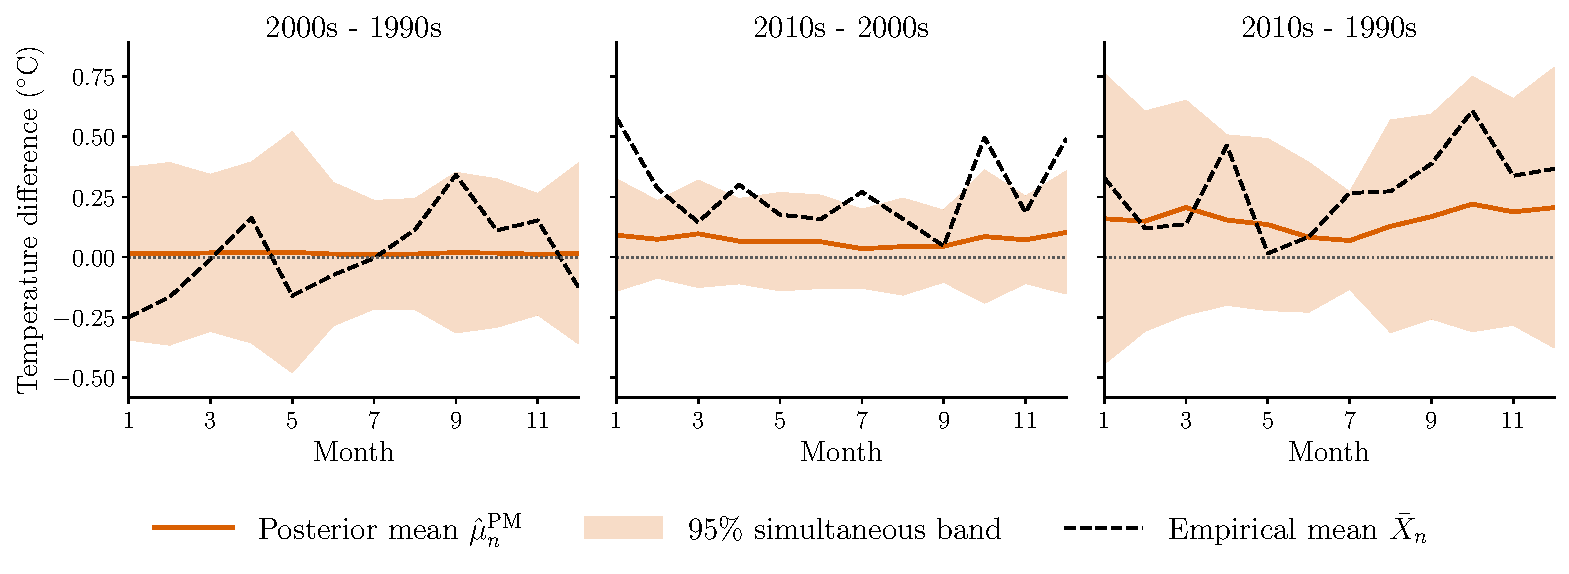
\includegraphics[width=.99\textwidth]{figures/real_climate_posterior.pdf}
  \caption{Estimated posterior mean and 95\% simultaneous credible bands given by our RKBT test for the three pairwise-difference temperature data sets. The empirical mean is also shown for reference.}\label{fig:climate_posterior}
\end{figure}


\section{Discussion}\label{sec:conclusions}

In this work we have described a Bayesian test for the mean \(\mu\) of a Gaussian process, observed through i.i.d.\ functional samples. The proposed model hinges on a finite-dimensional representation enabled by the reasonable assumption that \(\mu\in\Hcal(K)\), where \(\Hcal(K)\) is the RKHS associated with the covariance function \(K\) of the process. The case \(\mu\notin \Hcal(K)\), though not treated here, is also interesting in its own right. When the true mean function \(\mu_*\) lies outside \(\Hcal(K)\), by the Feldman--Hájek dichotomy the measures \(\pp_{\mu_*}\) and \(\pp_0\) are mutually singular, so there exists a Borel set \(S\) such that \(\pp_{\mu_*}(S)=1\) and \(\pp_0(S)=0\). In principle, we could define the test \(\phi(X)=\mathds{1}\{X\in S\}\), which has both type I and type II errors equal to 0, and can separate \(\pp_{\mu_*}\) and \(\pp_0\) perfectly with a single full observation of the process. This is an example of a ``near-perfect'' testing situation, in which the functional nature of the data allows exact verification of the null hypothesis in theory; in a discretized setting this effect might not be detectable with a finite grid, but it can manifest as the grid becomes dense \citep{torrecilla2020optimal}. Other instances of this phenomenon applied to functional data classification are studied, for example, by \citet{delaigle2012achieving} or \citet{berrendero2018use}. 

The Bayesian formulation of the test is flexible enough to accommodate a range of priors, fixing only the so-called ``local'' spike-and-slab prior on the coefficient vector \(b\), which is a common choice in multivariate settings. Other authors \citep[e.g.][]{johnson2010use} have objected to local alternative priors on a philosophical level, proposing different nonlocal alternatives. However, adopting them in our context would render the closed-form marginalization of \(b\) invalid, which is central to our computational strategy. Our approach connects the functional testing problem to a variable-dimension model in a principled way, and is theoretically backed by near-optimal posterior consistency results. These findings confirm that the Bayes factor-based test is asymptotically reliable under both the null and the alternative, and they provide a more refined description of how quickly evidence accumulates in favor of the correct hypothesis. This analysis is complemented by numerical studies with a tractable computational paradigm, showing that our test is on a par with other methods in the literature. Lastly, we have also illustrated how the Bayesian aspect of the model can be used to quantify the uncertainty in the posterior distribution and interpret the results of the test, since we have access to a continuous posterior probability that measures the strength of evidence against the null.

We believe that this Bayesian framework opens several compelling paths for future research, demonstrating the practical and theoretical utility of RKHS representations in managing the inherent infinite-dimensionality of functional data. In particular, exploring the role of impact points within the RKHS approximation could yield meaningful new methodologies for change-point detection or variable selection in functional estimation. Furthermore, to our knowledge, the trans-dimensional aspect of the posterior approximation through RJMCMC---together with previous work by \citet{berrendero2025bayesian}---is a novel contribution in functional data.


%*****************************************
%*****************************************
%*****************************************
%*****************************************
%*****************************************
